
\section{Полосы равной толщины и равного наклона. Интерференция света на тонких пленках. Кольца Ньютона.}

\subsection{Интерференция волн при отражении от пластины. Полосы равного наклона.}

Пусть луч падает на плоскопараллельную пластину толщиной  $h$ с показателем преломления $n$ под некоторым углом $\alpha$ к нормали. Этот луч может сразу отразиться от верхней поверхности (порождая луч 1), а может сначала попасть внутрь пластины, а затем, отразившись от нижней грани, выйти из пластины через верхнюю поверхность (порождая луч 2). В результате каждый луч расщепляется на два, которые могут интерферировать между собой.
\begin{figure}[h!]
    \centering
    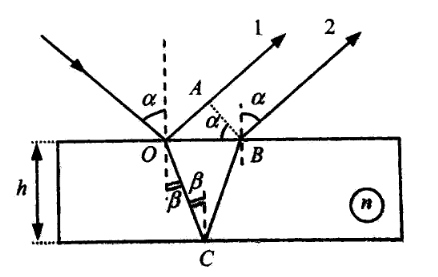
\includegraphics[scale=1]{plas.png}
    \caption{К расчету интерференции волн при отражении от пластины}
    \label{fig:my_label}
\end{figure} 

\bigskip

Найдем оптическую разность хода лучей 1 и 2. Проведем отрезок $AB$ перпендикулярно лучам 1 и 2. Тогда искомая длина набирается на трассах лучей до их пересечения с отрезком $AB$ и составляет

\begin{equation*}
    \delta_1 = L_2 - L_1 = n\cdot OCB - OA.
\end{equation*}

Длина трассы луча 2 в пластине составляет

\begin{equation*}
    OCB = \frac{2h}{\cos\beta},
\end{equation*}
где $beta$ - угол преломления, даваемый законом Снеллиуса:

\begin{equation*}
    \sin\alpha = n\sin\beta.
\end{equation*}


Для нахождения длины отрезка $OA$ найдем горизонтальный ход луча 2 в пластине:

 \begin{equation*}
     OB = 2h\tan\beta .
 \end{equation*}

Отсюда следует

 \begin{equation*}
     OA = OB\sin\alpha = 2h\tan\beta\sin\alpha .
 \end{equation*}
Таким образом, получаем
 \begin{equation*}
     \delta_1 = n\frac{2h}{\cos\beta} - 2h\tan\beta\sin\alpha = \frac{2hn}{\cos\beta}\left(1 - \frac{1}{n}\sin\beta\sin\alpha\right).
 \end{equation*}
С помощью закона Снеллиуса отсюда находим


 \begin{equation*}
    \delta_1 = 2hn\cos\beta = 2h\sqrt{n^2 - \sin^2\alpha}.
 \end{equation*}


Помимо полученной разности хода вклад в сдвиг фаз лучей может давать и отражение от поверхностей. Согласно формулам Френеля амплитудный коэффициент отражения при нормальном падении волны равен

\begin{equation*}
    r = \frac{E_{\text{отр}}}{E_{\text{пад}}} = \frac{1-n}{1+n}
\end{equation*}
 
 
 Следовательно, фаза волны меняется на $\pi $ при отражении от среды оптически более плотной и не меняется при отражении от среды оптически менее плотной. Такая же ситуация имеет место для $s-$поляризованной волны при падении под любыми углами. Для $p-$ поляризованной волны изменение фазы на $\pi$ имеет место для углов падения, не превышающих угла Брюстера. При больших же углах фаза волны не меняется.
 
 Таким образом, если угол падения не превышает угла Брюстера, то из найденной разности хода лучей $\delta$ следует вычесть поправку $\frac{\lambda}{2}$, обусловленную отражением луча 1 от оптически более плотной среды:
 
 \begin{equation*}
     \delta = \delta_1 - \frac{\lambda}{2}
 \end{equation*}
 
 Интерференционные максимумф интенсивности должны наблюдаться, если $\delta = m\lambda$, m = 0,1,2,..., или
 
\begin{equation*}
    2h\sqrt{n^2- \sin^2\alpha} = \left(m+\frac{1}{2}\right)\lambda .
\end{equation*}

Это равенство выделяет те углы падения лучей, при которых волны благодаря интерференции усиливаются. Если же выполняется условие $\delta = \left(m+\frac{1}{2}\right)\lambda$, или

\begin{equation*}
    2h\sqrt{n^2- \sin^2\alpha} = m\lambda ,
\end{equation*}

то происходит интерференционное гашение волн.

\medskip

Для наблюдения интерференционных полос на пути отраженных лучей следует поставить собирающую линзу.
Известно, что линза собирает параллельный пучок лучей в точку в фокальноф плоскости. Эта точка (в случае тонкой линзы) находится на пересечении фокальной плоскости с лучом, параллельным пучку и проходящим через оптический центр линзы. В зависимости от угла падения на пластину отраженные лучи будут собираться в разных точках фокальной плоскости. Пусть падающий на пластинку свет имеет разные направления (рассеяный свет). Тогда для лучей с направлениями, отвечающими интерференционному усилению, будут наблюдаться светлые полосы. Лучи же, для которых имеет место интерференционное подавление, будут на экране формировать темные полосы.


\begin{figure}[h!]
    \centering
    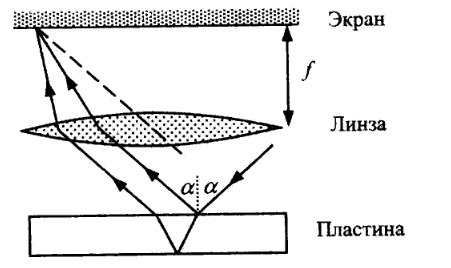
\includegraphics[scale=1]{plas2.png}
    \caption{Схема наблюдения интерференционных полос равного наклона при отражении света от пластины}
    \label{fig:my_label}
\end{figure} 
Поскольку в данном эксперименте каждая из полос формируется только группой лучей с одним и тем же углом падения (наклона), то такии линии на экране называются \textit{полосами равного наклона}.
\subsection{Полосы равного наклона}
\subsection{Кольца Ньютона}

Схема опыта: свет падает на линзу с большим радиусом кривизны, лежащую на плоскопараллельной стеклянной пластинке. Регистрируется излучение, отраженное системой или прошедшее через нее. Оказалось, что при нормальном падении света на сферической поверхности локализована серия колец - интерференционных полос.


\begin{figure}[h!]
    \centering
    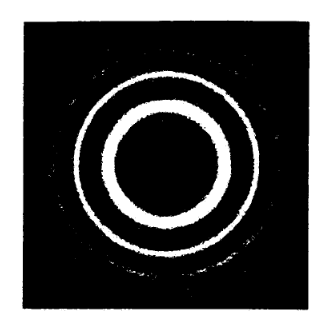
\includegraphics[scale=1]{anal_rings2.png}
    \caption{Кольца Ньютона в отраженном свете}
    \label{fig:my_label}
\end{figure} 

Зазор между линзой и пластинкой играет роль, аналогичную клину. Интерференция возникает между лучами, отраженными от пластинки и от кривой поверхности линзы. Разность хода отраженных лучей зависит от толщины зазора $d$ в месте падения луча 1 и составляет $2d$. Найдем ее.

\bigskip



\begin{figure}[h!]
    \centering
    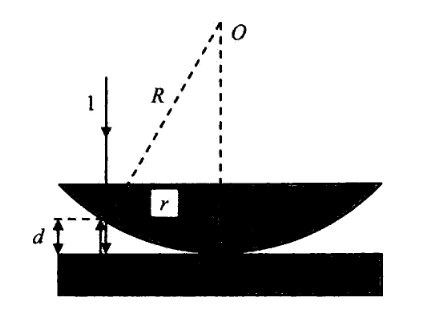
\includegraphics[scale=1]{anal_rings1.png}
    \caption{Схема оптической системы, в которой наблюдаются кольца Ньютона}
    \label{fig:my_label}
\end{figure} 
Пусть радиус кривизны линзы равен $R$. Тогда из теоремы Пифагора находим

\begin{equation*}
    R^2 = r^2 + (R-d)^2 \Rightarrow 2Rd = r^2/
\end{equation*}

Здесь, считая зазор тонким в области наблюдения, мы пренебрегли малой величиной $d^2$ по сравнению с удержанными слагаемыми. При отражении луча от оптически более плотной среды волны приобретает дополнительный сдвиг фазы,  соответствующий дополнительной разности хода $\frac{\lambda}{2}$. Поэтому находим оптическую разность хода лучей, отраженных от линзы и пластинки:

\begin{equation*}
    \Delta = 2d + \frac{\lambda}{2} = \frac{r^2}{R} + \frac{\lambda}{2}.
\end{equation*}

Темные кольца отвечают интерференционным минимумам интенсивности, наблюдающимся при условии $\Delta = (m+1/2)\lambda$, откуда находим радиусы темных колец:

\begin{equation*}
    r_m = \sqrt{m\lambda R}, \hspace{10px} m = 0,1,2,...
\end{equation*}

Из условия $\Delta = m\lambda$ получаем радиусы светлых колец:

\begin{equation*}
    r_m = \sqrt{(m-1/2)\lambda R}, \hspace{10px} m = 1,2,...
\end{equation*}

Таким образом, в отраженном свете центр колец темный. Если бы мы рассматривали прошедший свет, то добавка $\frac{\lambda}{2}$ к разности хода не возникала вследствии того, что отраждение луча от оптически более плотной среды двукратное. Соответственно темные и светлые кольца меняются местами, причем центр колец оказывается светлым.

В заключение можно отметить следующее:

\begin{enumerate}
    \item Наблюдающиеся кольца являются полосами \textit{равной толщины}, поскольку их положение зависит от толщины зазора: волны, проходящие участки зазора, имеющие одну и ту же толщину, но в разных точках вокруг оси системы, образуют одно кольцо.
    \item Радиусы колец зависят от длины волны. В случае немонохроматического света каждое кольцо будет иметь различную окраску в разных его точках: в точках, более удаленных от центра, окраска смещается в красную область спектра.
    \item В расчетах выше показатель преломления между линзой и пластинкой был равен единице. Если это не так, будет меняться разность хода отраженных лучей, приводя к изменению радиусов колец Ньютона.
    \item Кольца Ньютона используются для измерения радиусов кривизны поверхностей, длин волн света и показателей преломления.
\end{enumerate}

